\chapter{User Interface}
\label{chap:UI}

\section{Design}

\begin{figure}[h]
    \centering
    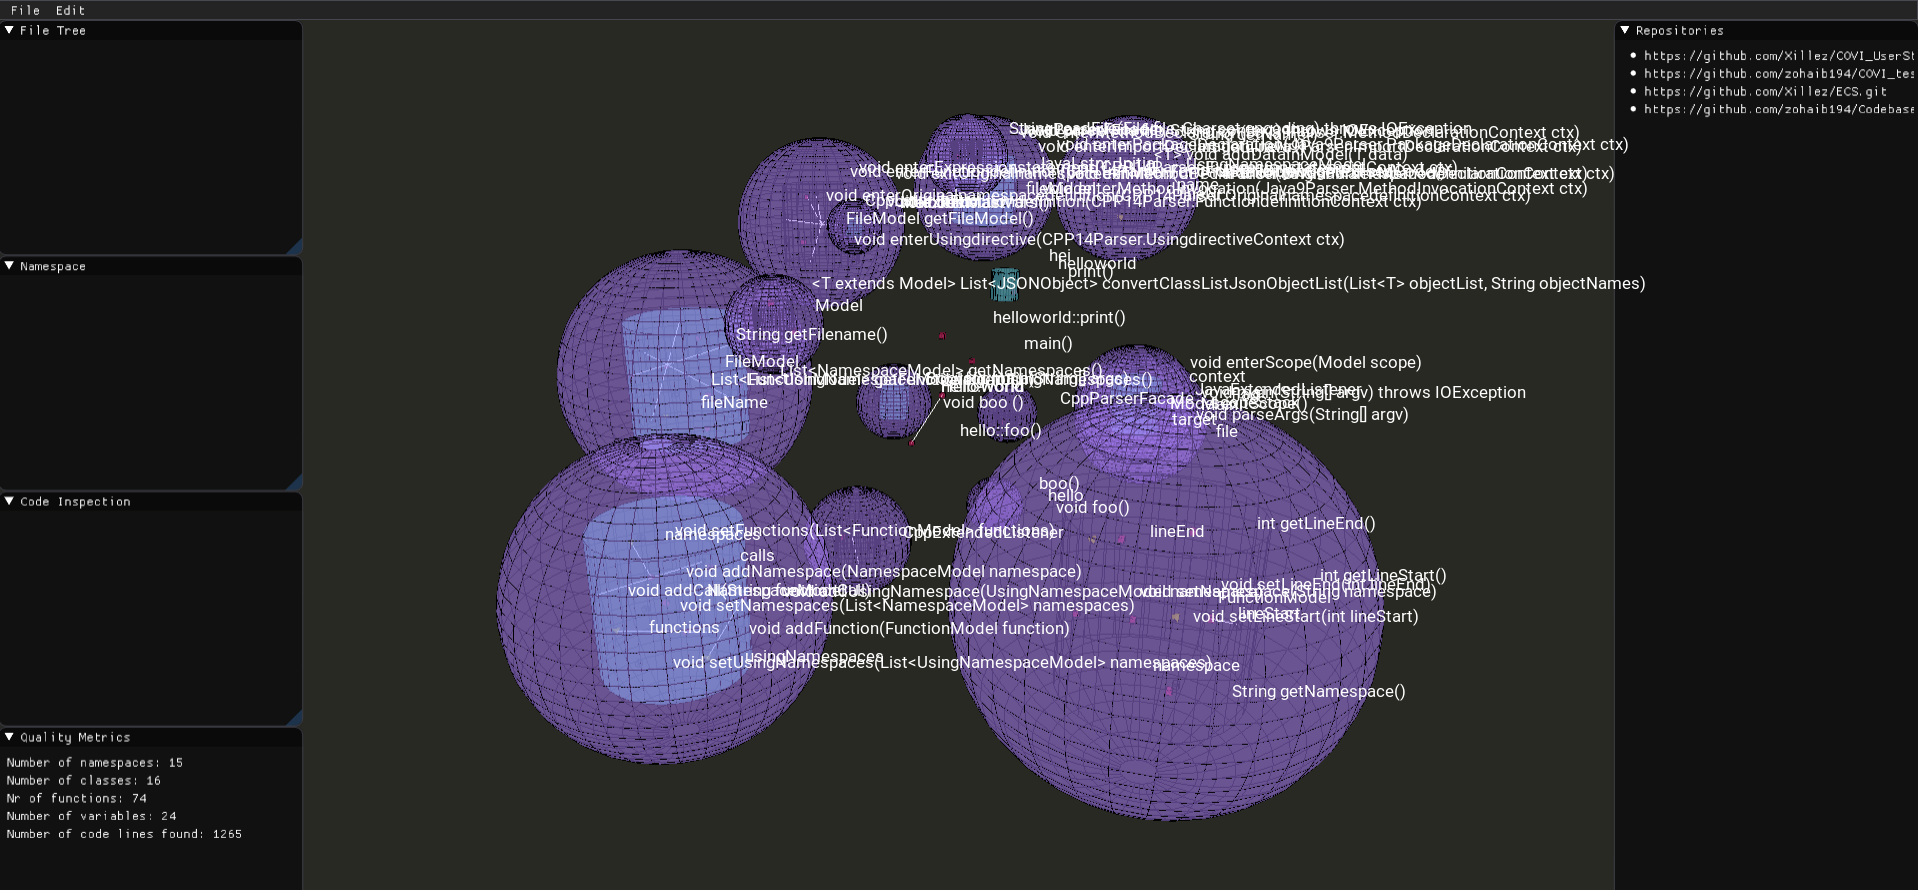
\includegraphics[width=\textwidth]{inc/images/COVI_Visualization.png}
    \caption{Final UI layout.}
    \label{fig:finalui}
\end{figure}

The initial \gls{ui} concept shown in appendix \ref{app:initialConcept}, was presented to product owner during the seconded meeting to visualize how the team had thought of design layout of the system. Product owner was pleased by the looks of the system and approved it.

Visualization was inspired by tensorflow. Tensorflow deals with concepts like AI and big data and where they have very understandable and readable ways to visualize a big set of data through graphs. The team wanted an intuitive way of visualizing the data-structure and along with keeping the concepts like loosely or highly coupled relation in the visualization. Therefore tensorflow inspiration seemed a perfect way to tackle this problem.

The left side of the figure \ref{app:initialConcept}, is used to show project related data such as file structure, namespaces, implementation and quality metrics. Whilst the right side is used to show unrelated data such as repositories registered in the system for easy switching between repositories. 

The final \gls{ui} layout is shown in figure \ref{fig:finalui}. This 
























